\setcounter{equation}{0}

\chapter{Introduction}

\noindent In the rapidly evolving landscape of financial technology, efficient and secure transaction processing is paramount. The integration of advanced technologies such as Large Language Models (LLMs) into financial systems represents a significant leap forward in enhancing transaction management, user interaction, and overall financial operations. This project aims to develop a robust LLM-based system that processes various transaction-related queries, offering an intuitive, efficient, and secure solution for managing financial transactions.

\noindent This project addresses the common challenges in transaction processing, such as inefficiency, complexity, and security vulnerabilities. By leveraging the capabilities of LLMs, our system aims to streamline transaction workflows, provide clear and concise responses to user queries, and enforce strict security protocols to protect sensitive financial data.

\begin{figure}[h!]
    \centering
{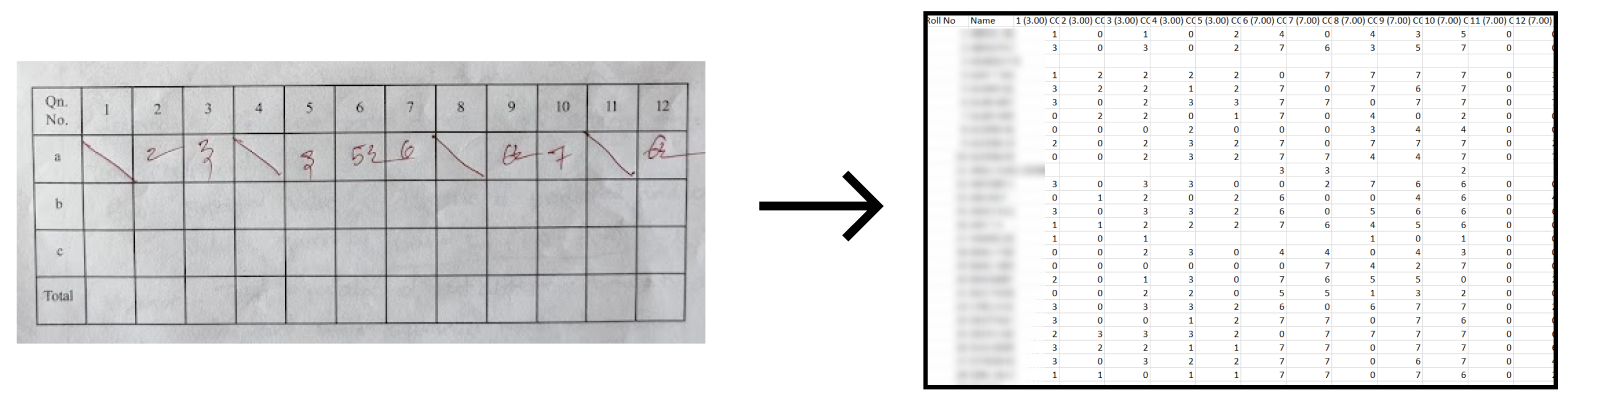
\includegraphics[width=0.9\textwidth]{Images/Intro/intro_pic.jpg}}
  \caption{Handwritten Text to Digital Text}
\end{figure}

\clearpage

\section{Background}

\noindent The financial services industry has seen remarkable transformations over the past few decades, driven by technological advancements and the growing demand for digital solutions. Traditional transaction processing systems, while reliable, often struggle to meet the dynamic needs of modern users. These systems typically involve complex interfaces and manual processes, which can lead to inefficiencies and user frustration. The need for more adaptive, responsive, and user-friendly financial tools has never been greater.

\noindent Large Language Models, such as OpenAI's GPT-3 and Google's BERT, have revolutionized the field of natural language processing (NLP). These models are designed to understand and generate human-like text, making them exceptionally well-suited for applications that require nuanced language comprehension. Their ability to handle diverse and complex queries makes them ideal for integration into transaction processing systems, where user inputs can vary widely in form and intent.

\noindent The potential of LLMs to transform transaction processing lies in their capability to interpret natural language queries accurately and provide relevant responses. Unlike traditional systems that rely on predefined commands and rigid protocols, LLMs can adapt to a wide range of user inputs, offering a more flexible and intuitive interface. This adaptability is crucial for catering to users with varying levels of technical expertise and financial literacy.

\noindent Furthermore, the integration of LLMs into financial systems can significantly enhance data processing and decision-making. By leveraging the deep learning capabilities of these models, financial institutions can analyze large volumes of transaction data more effectively, identifying patterns and insights that would be challenging to uncover using conventional methods. This ability to derive actionable insights from data can drive better financial strategies and outcomes.

\clearpage

\section{Motivation}

\noindent The primary motivation for this project is to address the limitations of current financial transaction systems and meet the evolving needs of users. Today's users expect seamless, efficient, and secure interactions with their financial institutions. However, the complexity of existing systems often results in a steep learning curve and increased potential for errors. By integrating LLMs, we aim to simplify these interactions, making them more intuitive and user-friendly.


\noindent Security is another critical factor driving this project. Financial transactions involve sensitive data, and ensuring the security of this data is paramount. Traditional systems often face challenges in implementing robust security measures without compromising usability. Our project incorporates advanced user permission protocols to ensure that only authorized users can perform specific actions, thereby enhancing the overall security of financial transactions.

\noindent Additionally, the growing volume of financial transactions necessitates more efficient processing mechanisms. Manual and semi-automated processes can no longer keep pace with the demand for real-time transaction processing. By automating query handling and transaction execution through LLMs, we can significantly reduce processing times and improve operational efficiency, benefiting both financial institutions and their customers.

\noindent Lastly,the project is motivated by the potential to leverage advanced AI technologies to create a more inclusive financial ecosystem. Many users, particularly those with limited technical skills or disabilities, struggle to navigate traditional financial interfaces. By providing a natural language interface, we aim to make financial services more accessible, enabling a broader demographic to manage their finances effectively and independently.

\noindent The integration of Large Language Models into financial transaction processing systems holds significant promise for improving user experience, enhancing security, and increasing operational efficiency. By addressing current limitations and leveraging cutting-edge AI technologies, this project aims to set a new standard in the financial industry, ultimately contributing to a more efficient and inclusive financial ecosystem.

\clearpage

\section{Objective and Scope}

\subsection{Objective}

The primary objective of this project is to develop an advanced transaction processing system that leverages Large Language Models (LLMs) to provide a seamless, efficient, and secure user experience. This system aims to understand and process natural language queries related to financial transactions, such as retrieving transaction totals, executing transactions, and calculating cash transfers. By integrating LLMs, the project seeks to simplify user interactions with financial systems, making them more intuitive and accessible. Additionally, the project aims to enhance security through robust user permission protocols, ensuring that only authorized users can perform specific actions. Ultimately, this project aspires to set a new standard in transaction processing by combining cutting-edge AI technology with stringent security measures, thereby improving operational efficiency and user satisfaction.

\subsection{Scope}

The scope of this project encompasses the design, development, and deployment of an LLM-based transaction processing system. The system will include several core components: a natural language interface for user queries, a processing engine powered by a Large Language Model, an action model to execute transactions, and a secure storage bucket for data management. The project will involve the implementation of advanced natural language processing techniques to ensure accurate interpretation and response to user queries.

\noindent Additionally, the system will integrate user permission protocols to control access to various functionalities, enhancing security and compliance. The project will also include rigorous testing phases to validate the system's performance, accuracy, and security. Furthermore, the scope extends to the development of a scalable architecture capable of handling increased user loads and transaction volumes. This comprehensive approach aims to deliver a robust, efficient, and user-friendly transaction processing solution that meets the evolving needs of modern financial systems.

\clearpage

\noindent As a result, the developed system is expected to significantly enhance the efficiency and user experience of financial transaction processing. By providing a natural language interface, users will be able to interact with the system in a more intuitive and accessible manner, reducing the learning curve and minimizing errors. The integration of LLMs will ensure that user queries are accurately understood and addressed, while the implementation of robust security measures will protect sensitive financial data and transactions from unauthorized access. The scalable architecture will enable the system to accommodate growing user bases and transaction volumes, ensuring reliability and performance even under high demand. Ultimately, this project aims to set a new standard in financial technology by delivering a solution that combines cutting-edge AI capabilities with stringent security protocols and exceptional user experience.

\section{Contributions}

\noindent This project makes a significant contribution to financial technology by leveraging Large Language Models (LLMs) to create an intuitive and user-friendly transaction processing system. By allowing users to interact with the system using natural language, it reduces the complexity of financial transactions and makes financial management more accessible to a wider audience, enhancing overall user experience.

\noindent In addition to improving usability, the project enhances security through the implementation of robust user permission protocols. These protocols ensure that only authorized users can perform specific actions, thereby protecting sensitive financial data and operations. This focus on security is crucial in mitigating the risks associated with increasingly sophisticated cyber threats.

\noindent Furthermore, the project contributes to operational efficiency by automating the processing and execution of transaction queries. This automation reduces the need for manual intervention, resulting in faster transaction processing and lower operational costs. These efficiency gains benefit both financial institutions and their customers, leading to quicker service delivery and improved satisfaction.